\documentclass{article}
\usepackage{amsmath}
\usepackage{tikz}
\usetikzlibrary{matrix}

\begin{document}

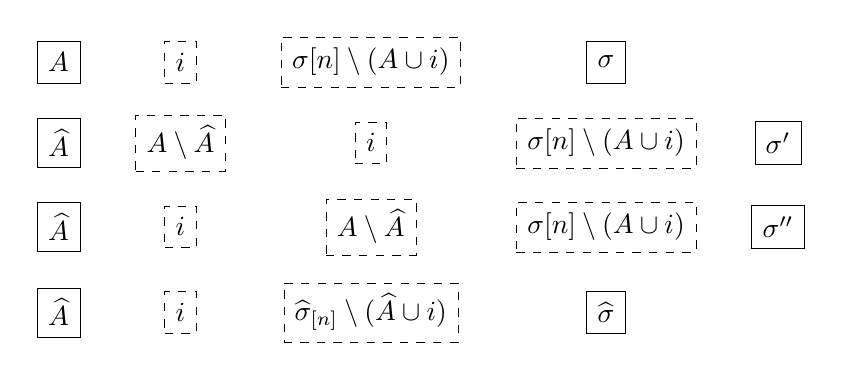
\begin{tikzpicture}[every node/.style={anchor=center}]
  \matrix (m) [matrix of math nodes,
               column sep=2em,
               row sep=1em,
               nodes={minimum height=1.5em, inner sep=4pt},
               row 1/.style={nodes={draw, ultra thin}},
               row 2/.style={nodes={draw, ultra thin}},
               row 3/.style={nodes={draw, ultra thin}},
               row 4/.style={nodes={draw, ultra thin}}
              ]
  {
    A & |[dashed]| i & |[dashed]| \sigma[n]\setminus(A\cup i) & \sigma \\
    \widehat{A} & |[dashed]| A\setminus\widehat{A} & |[dashed]| i & |[dashed]| \sigma[n]\setminus(A\cup i) & \sigma' \\
    \widehat{A} & |[dashed]| i & |[dashed]| A\setminus\widehat{A} & |[dashed]| \sigma[n]\setminus(A\cup i) & \sigma'' \\
    \widehat{A} & |[dashed]| i & |[dashed]| \widehat{\sigma}_{[n]}\setminus(\widehat{A}\cup i) & \widehat{\sigma} \\
  };
\end{tikzpicture}

\end{document}